\documentclass{beamer}

\usetheme{metropolis}

\usepackage{pgfplots}
\usepackage{hyperref}
\usepackage{listings}
\usepackage{tcolorbox}
\usepackage{xcolor}

\usepgfplotslibrary{groupplots}

\usetikzlibrary{calc}

\hypersetup{
    colorlinks=true,
    linkcolor=blue,
    urlcolor=blue!80
}

\lstdefinestyle{RStyle}{
    language=R,
    basicstyle=\ttfamily\fontsize{5}{6}\selectfont,
    keywordstyle=\color[RGB]{17, 115, 187},
    commentstyle=\color[RGB]{0, 128, 0},
    identifierstyle=\color[RGB]{0, 0, 0},
    stringstyle=\color[RGB]{205, 49, 49},
    numberstyle=\fontsize{5}{6}\selectfont\color[RGB]{128, 128, 128},
    numbers=left,
    numbersep=6pt,
    backgroundcolor=\color[RGB]{255, 255, 255},
    frame=single,
    rulecolor=\color[RGB]{0, 0, 0},
    showstringspaces=false,
    breaklines,
    xleftmargin=3pt,
    xrightmargin=3pt,
    framesep=3pt,
    aboveskip=-1.5pt,
    belowskip=-0.5pt,
    showlines=true
}

\lstdefinestyle{PythonStyle}{
    language=Python,
    basicstyle=\ttfamily\fontsize{5}{6}\selectfont,
    keywordstyle=\color[RGB]{26, 13, 171},
    commentstyle=\color[RGB]{0, 128, 0},
    identifierstyle=\color[RGB]{0, 0, 0},
    stringstyle=\color[RGB]{205, 49, 49},
    numberstyle=\fontsize{5}{6}\selectfont\color[RGB]{128, 128, 128},
    frame=tblr,
    backgroundcolor=\color[RGB]{245, 245, 245},
    rulecolor=\color[RGB]{192, 192, 192},
    showstringspaces=false,
    breaklines,
    xleftmargin=3pt,
    xrightmargin=3pt,
    framesep=3pt,
    aboveskip=-1.5pt,
    belowskip=-0.5pt,
    showlines=true,
}

\lstdefinestyle{ROutput}{
    language=R,
    basicstyle=\ttfamily\fontsize{5}{6}\selectfont,
    backgroundcolor=\color[RGB]{255, 255, 255},
    commentstyle=\color[HTML]{009900},
    stringstyle=\color[HTML]{0000FF},
    keywordstyle=\color[HTML]{000000},
    numberstyle=\tiny\color[HTML]{000000},
    breakatwhitespace=true,
    breaklines=true,
    frame=single,
    rulecolor=\color{black},
    showstringspaces=false,
    breaklines,
    xleftmargin=3pt,
    xrightmargin=3pt,
    framesep=3pt,
    aboveskip=-1.5pt,
    belowskip=-0.5pt,
    showlines=true
}

\lstdefinestyle{PythonOutput}{
    basicstyle=\fontsize{5}{6}\selectfont,
    backgroundcolor=\color[RGB]{255, 255, 255},
    rulecolor=\color[RGB]{192, 192, 192},
    frame=single,
    numbers=none,
    showstringspaces=false,
    breaklines=true,
    breakatwhitespace=true,
    showstringspaces=false,
    breaklines,
    xleftmargin=3pt,
    xrightmargin=3pt,
    framesep=3pt,
    aboveskip=-1.5pt,
    belowskip=-0.5pt,
    showlines=true,
    keywordstyle=\color[RGB]{255, 0, 0},
    morekeywords={AttributeError}
}

\title{PSY9511: Seminar 3}
\subtitle{Variable selection and regularization}
\author{Esten H. Leonardsen}
\date{07.09.23}

\begin{document}
	\begin{frame}
	 	\maketitle
	\end{frame}

    \begin{frame}{Outline}
        \centering
        \vfill
        \begin{enumerate}
            \item Introduction
            \begin{itemize}
                \item Python
                \item Coding tips: Separation of concerns
            \end{itemize}
            \item Variable selection
            \begin{itemize}
                \item Best subset selection
                \item Forward stepwise selection
                \item Backward stepwise selection
            \end{itemize}
            \item Regularization
            \begin{itemize}
                \item Ridge regression
                \item Lasso
                \item Elastic net
            \end{itemize}
            \item Dimensionality reduction
            \begin{itemize}
                \item Principal component regression
                \item Partial least squares
            \end{itemize}
        \end{enumerate}
        \vfill
    \end{frame}

    \def\codewidth{4.5cm}

    \begin{frame}[fragile]{Python: Imports} % R import
        \centering
        \vfill
        \begin{tikzpicture}
            \node[
                minimum width=\codewidth,
                text width=\codewidth,
                align=left,
                inner sep=0pt,
                outer sep=0pt,
                draw=black
            ] (rcode) at (0, 0) {
                \begin{lstlisting}[style=RStyle, linewidth=\codewidth]




                \end{lstlisting}
            };

            \node[
                draw=black,
                dashed,
                minimum width=\codewidth,
                minimum height=2cm,
                anchor=north,
                text width=\codewidth * 0.98,
                text depth=1.6cm,
                inner sep=0pt,
                outer sep=0pt
            ] (mass) at ($ (rcode.south) - (0, 1.5) $) {\footnotesize{\textbf{MASS}}};

            \node[
                draw=black,
                dashed,
                inner sep=3pt
            ] at (mass) {\scriptsize{lda}};


            \node[] at (-2.35, 0.53) {};
            \node[] at (8.08, -4) {};
        \end{tikzpicture}
        \vfill
    \end{frame}

    \begin{frame}[fragile]{Python: Imports} % R import
        \centering
        \vfill
        \begin{tikzpicture}
            \node[
                minimum width=\codewidth,
                text width=\codewidth,
                align=left,
                inner sep=0pt,
                outer sep=0pt,
                draw=black
            ] (rcode) at (0, 0) {
                \begin{lstlisting}[style=RStyle, linewidth=\codewidth]
library(MASS)



                \end{lstlisting}
            };

            \node[
                draw=black,
                dashed,
                minimum width=\codewidth,
                minimum height=2cm,
                anchor=north,
                text width=\codewidth * 0.98,
                text depth=1.6cm,
                inner sep=0pt,
                outer sep=0pt
            ] (mass) at ($ (rcode.south) - (0, 1.5) $) {\footnotesize{\textbf{MASS}}};

            \node[
                draw=black,
                dashed,
                inner sep=3pt
            ] at (mass) {\scriptsize{lda}};


            \draw[->] (mass.north) -- (rcode.south);
            \node[] at (-2.35, 0.53) {};
            \node[] at (8.08, -4) {};
        \end{tikzpicture}
        \vfill
    \end{frame}

    \begin{frame}[fragile]{Python: Imports} % R import and usage
        \centering
        \vfill
        \begin{tikzpicture}
            \node[
                minimum width=\codewidth,
                text width=\codewidth,
                align=left,
                inner sep=0pt,
                outer sep=0pt,
                draw=black
            ] (rcode) at (0, 0) {
                \begin{lstlisting}[style=RStyle, linewidth=\codewidth]
library(MASS)

lda_fit <- lda(display ~ age + fb,
               data = display)
                \end{lstlisting}
            };

            \node[
                draw=black,
                dashed,
                minimum width=\codewidth,
                minimum height=2cm,
                anchor=north,
                text width=\codewidth * 0.98,
                text depth=1.6cm,
                inner sep=0pt,
                outer sep=0pt
            ] (mass) at ($ (rcode.south) - (0, 1.5) $) {\footnotesize{\textbf{MASS}}};

            \node[
                draw=black,
                dashed,
                inner sep=3pt
            ] at (mass) {\scriptsize{lda}};


            \draw[->] (mass.north) -- (rcode.south);
            \node[] at (-2.35, 0.53) {};
            \node[] at (8.08, -4) {};
        \end{tikzpicture}
        \vfill
    \end{frame}

    \begin{frame}[fragile]{Python: Imports} % Import everything from package
        \centering
        \vfill
        \begin{tikzpicture}
            \node[
                minimum width=\codewidth,
                text width=\codewidth,
                align=left,
                inner sep=0pt,
                outer sep=0pt,
                draw=black
            ] (rcode) at (0, 0) {
                \begin{lstlisting}[style=RStyle, linewidth=\codewidth]
library(MASS)

lda_fit <- lda(display ~ age + fb,
               data = display)
                \end{lstlisting}
            };
            \node[
                minimum width=\codewidth,
                text width=\codewidth,
                align=left,
                inner sep=0pt,
                outer sep=0pt,
                anchor=north west,
                draw=black,
                label={[blue,
                        anchor=north east,
                        font=\ttfamily\fontsize{5}{6}\selectfont,
                        inner sep=0pt,
                        outer sep=0pt,
                        xshift=-3pt,
                        yshift=-3pt,
                        text depth=0
                       ]north west:In{[}1{]}:},
            ] (pythoncode) at ($ (rcode.north east) + (1.4, 0) $) {
                \begin{lstlisting}[style=PythonStyle, linewidth=\codewidth]
from sklearn import *

lda = discriminant_analysis.LinearDiscriminantAnalysis()
lda.fit(display[['age', 'fb']],
        display['display'])
                \end{lstlisting}
            };

            \node[
                draw=black,
                dashed,
                minimum width=\codewidth,
                minimum height=2cm,
                anchor=north,
                text width=\codewidth * 0.98,
                text depth=1.6cm,
                inner sep=0pt,
                outer sep=0pt
            ] (mass) at ($ (rcode.south) - (0, 1.5) $) {\footnotesize{\textbf{MASS}}};

            \node[
                draw=black,
                dashed,
                inner sep=3pt
            ] at (mass) {\scriptsize{lda}};

            \node[
                draw=black,
                dashed,
                minimum width=\codewidth,
                minimum height=2cm,
                anchor=west,
                text width=\codewidth * 0.98,
                text depth=1.6cm,
                inner sep=0pt,
                outer sep=0pt,
            ] (sklearn) at ($ (mass.east) + (1.4, 0) $) {\footnotesize{\textbf{sklearn}}};

            \node[
                draw=black,
                dashed,
                minimum width=\codewidth * 0.8,
                minimum height=1.3cm,
                text width=\codewidth * 0.78,
                text depth=0.97cm,
                inner sep=0pt,
                outer sep=0pt,
                anchor=south
            ] (da) at ($ (sklearn.south) + (0, 0.15) $) {\scriptsize{\textbf{discriminant\_analysis}}};

            \node[
                draw=black,
                dashed,
                inner sep=2pt,
                anchor=south
            ] (lda) at ($ (da.south) + (0, 0.15) $) {\tiny{LinearDiscriminantAnalysis}};

            \draw[->] (mass.north) -- (rcode.south);
            \draw[->] (sklearn.north) -- (pythoncode.south);
            \node[] at (-2.35, 0.53) {};
            \node[] at (8.08, -4) {};
        \end{tikzpicture}
        \vfill
    \end{frame}

    \begin{frame}[fragile]{Python: Imports} % Import entire package
        \centering
        \vfill
        \begin{tikzpicture}
            \node[
                minimum width=\codewidth,
                text width=\codewidth,
                align=left,
                inner sep=0pt,
                outer sep=0pt,
                draw=black
            ] (rcode) at (0, 0) {
                \begin{lstlisting}[style=RStyle, linewidth=\codewidth]
library(MASS)

lda_fit <- lda(display ~ age + fb,
               data = display)
                \end{lstlisting}
            };
            \node[
                minimum width=\codewidth,
                text width=\codewidth,
                align=left,
                inner sep=0pt,
                outer sep=0pt,
                anchor=north west,
                draw=black,
                label={[blue,
                        anchor=north east,
                        font=\ttfamily\fontsize{5}{6}\selectfont,
                        inner sep=0pt,
                        outer sep=0pt,
                        xshift=-3pt,
                        yshift=-3pt
                       ]north west:In{[}1{]}:},
            ] (pythoncode) at ($ (rcode.north east) + (1.4, 0) $) {
                \begin{lstlisting}[style=PythonStyle, linewidth=\codewidth]
import sklearn

lda = sklearn.discriminant_analysis.LinearDiscriminantAnalysis()
lda.fit(display[['age', 'fb']],
        display['display'])
                \end{lstlisting}
            };

            \node[
                draw=black,
                dashed,
                minimum width=\codewidth,
                minimum height=2cm,
                anchor=north,
                text width=\codewidth * 0.98,
                text depth=1.6cm,
                inner sep=0pt,
                outer sep=0pt
            ] (mass) at ($ (rcode.south) - (0, 1.5) $) {\footnotesize{\textbf{MASS}}};

            \node[
                draw=black,
                dashed,
                inner sep=3pt
            ] at (mass) {\scriptsize{lda}};

            \node[
                draw=black,
                dashed,
                minimum width=\codewidth,
                minimum height=2cm,
                anchor=west,
                text width=\codewidth * 0.98,
                text depth=1.6cm,
                inner sep=0pt,
                outer sep=0pt
            ] (sklearn) at ($ (mass.east) + (1.4, 0) $) {\footnotesize{\textbf{sklearn}}};

            \node[
                draw=black,
                dashed,
                minimum width=\codewidth * 0.8,
                minimum height=1.3cm,
                text width=\codewidth * 0.78,
                text depth=0.97cm,
                inner sep=0pt,
                outer sep=0pt,
                anchor=south
            ] (da) at ($ (sklearn.south) + (0, 0.15) $) {\scriptsize{\textbf{discriminant\_analysis}}};

            \node[
                draw=black,
                dashed,
                inner sep=2pt,
                anchor=south
            ] (lda) at ($ (da.south) + (0, 0.15) $) {\tiny{LinearDiscriminantAnalysis}};

            \draw[->] (mass.north) -- (rcode.south);
            \draw[->] (sklearn.north) -- (pythoncode.south);
            \draw[densely dotted] (lda.north) -- (sklearn.north);
            \node[] at (-2.35, 0.53) {};
            \node[] at (8.08, -4) {};
        \end{tikzpicture}
        \vfill
    \end{frame}

    \begin{frame}[fragile]{Python: Imports} % Proper import
        \centering
        \vfill
        \begin{tikzpicture}
            \node[
                minimum width=\codewidth,
                text width=\codewidth,
                align=left,
                inner sep=0pt,
                outer sep=0pt,
                draw=black
            ] (rcode) at (0, 0) {
                \begin{lstlisting}[style=RStyle, linewidth=\codewidth]
library(MASS)

lda_fit <- lda(display ~ age + fb,
               data = display)
                \end{lstlisting}
            };
            \node[
                minimum width=\codewidth,
                text width=\codewidth,
                align=left,
                inner sep=0pt,
                outer sep=0pt,
                anchor=north west,
                label={[blue,
                        anchor=north east,
                        font=\ttfamily\fontsize{5}{6}\selectfont,
                        inner sep=0pt,
                        outer sep=0pt,
                        xshift=-3pt,
                        yshift=-3pt
                       ]north west:In{[}1{]}:},
            ] (pythoncode) at ($ (rcode.north east) + (1.4, 0) $) {
                \begin{lstlisting}[style=PythonStyle, linewidth=\codewidth]
from sklearn.discriminant_analysis \
    import LinearDiscriminantAnalysis

lda = LinearDiscriminantAnalysis()
lda.fit(display[['age', 'fb']],
        display['display'])
                \end{lstlisting}
            };

            \node[
                draw=black,
                dashed,
                minimum width=\codewidth,
                minimum height=2cm,
                anchor=north,
                text width=\codewidth * 0.98,
                text depth=1.6cm,
                inner sep=0pt,
                outer sep=0pt
            ] (mass) at ($ (rcode.south) - (0, 1.5) $) {\footnotesize{\textbf{MASS}}};

            \node[
                draw=black,
                dashed,
                inner sep=3pt
            ] at (mass) {\scriptsize{lda}};

            \node[
                draw=black,
                dashed,
                minimum width=\codewidth,
                minimum height=2cm,
                anchor=west,
                text width=\codewidth * 0.98,
                text depth=1.6cm,
                inner sep=0pt,
                outer sep=0pt
            ] (sklearn) at ($ (mass.east) + (1.4, 0) $) {\footnotesize{\textbf{sklearn}}};

            \node[
                draw=black,
                dashed,
                minimum width=\codewidth * 0.8,
                minimum height=1.3cm,
                text width=\codewidth * 0.78,
                text depth=0.97cm,
                inner sep=0pt,
                outer sep=0pt,
                anchor=south
            ] (da) at ($ (sklearn.south) + (0, 0.15) $) {\scriptsize{\textbf{discriminant\_analysis}}};

            \node[
                draw=black,
                dashed,
                inner sep=2pt,
                anchor=south
            ] (lda) at ($ (da.south) + (0, 0.15) $) {\tiny{LinearDiscriminantAnalysis}};

            \draw[->] (mass.north) -- (rcode.south);
            \draw[->] (lda.north) -- (pythoncode.south);
            \node[] at (-2.35, 0.53) {};
            \node[] at (8.08, -4) {};
        \end{tikzpicture}
        \vfill
    \end{frame}

    \def\codewidth{4.8cm}

    \begin{frame}[fragile]{Python: pandas}
        \centering
        \vfill
        \begin{tikzpicture}
            \node[
                minimum width=\codewidth,
                text width=\codewidth,
                align=left,
                inner sep=0pt,
                outer sep=0pt,
                draw=black,
            ] (rcode) at (0, 0) {
                \begin{lstlisting}[style=RStyle]
path <- '/Users/esten/Downloads/Auto.csv'
df <- read.csv(path)
head(df, 10)
                \end{lstlisting}
            };
            \node[
                minimum width=\codewidth,
                text width=\codewidth,
                align=left,
                inner sep=0pt,
                outer sep=0pt,
                anchor=north west,
                draw=black,
                label={[blue,
                        anchor=north east,
                        font=\ttfamily\fontsize{5}{6}\selectfont,
                        inner sep=0pt,
                        outer sep=0pt,
                        xshift=-3pt,
                        yshift=-3pt
                       ]north west:In{[}1{]}:}
            ] (pythoncode) at ($ (rcode.north east) + (1.2, 0) $) {
                \begin{lstlisting}[style=PythonStyle]
import pandas as pd

path = '/Users/esten/Downloads/Auto.csv'
df = pd.read_csv(path)
df.head(10)
                \end{lstlisting}
            };

            \node[
                minimum width=\codewidth,
                text width=\codewidth,
                align=left,
                inner sep=0pt,
                outer sep=0pt,
                anchor=north,
            ] (routput) at ($ (rcode.south) - (0, 1) $) {
                \begin{lstlisting}[style=ROutput]
     mpg cylinders displacement horsepower
1    18         8        307.0        130
2    15         8        350.0        165
3    18         8        318.0        150
4    16         8        304.0        150
5    17         8        302.0        140
6    15         8        429.0        198
7    14         8        454.0        220
8    14         8        440.0        215
9    14         8        455.0        225
10   15         8        390.0        190
                \end{lstlisting}
            };

            \node[
                minimum width=\codewidth,
                text width=\codewidth,
                align=left,
                inner sep=0pt,
                outer sep=0pt,
                anchor=north west,
                label={[red,
                        anchor=north east,
                        font=\ttfamily\fontsize{5}{6}\selectfont,
                        inner sep=0pt,
                        outer sep=0pt,
                        xshift=-3pt,
                        yshift=-3pt
                        ]north west:Out{[}1{]}:}
            ] (pythonoutput) at ($ (routput.north east) + (1.2, 0) $) {
                \begin{lstlisting}[style=PythonOutput]
     mpg cylinders displacement horsepower
0    18         8        307.0        130
1    15         8        350.0        165
2    18         8        318.0        150
3    16         8        304.0        150
4    17         8        302.0        140
5    15         8        429.0        198
6    14         8        454.0        220
7    14         8        440.0        215
8    14         8        455.0        225
9    15         8        390.0        190
                \end{lstlisting}
            };
        \end{tikzpicture}
        \vfill
    \end{frame}

    \def\codewidth{9cm}

    \begin{frame}[fragile]{Python: numpy}
        \centering
        \vfill
        \begin{tikzpicture}
            \node[
                minimum width=\codewidth,
                text width=\codewidth,
                align=left,
                inner sep=0pt,
                outer sep=0pt,
                draw=black,
                label={[blue,
                        anchor=north east,
                        font=\ttfamily\fontsize{5}{6}\selectfont,
                        inner sep=0pt,
                        outer sep=0pt,
                        xshift=-3pt,
                        yshift=-3.5pt,
                        text depth=0
                       ]north west:In{[}1{]}:}
            ] (code0) at (0, 0) {
                \begin{lstlisting}[style=PythonStyle]
import numpy as np
                \end{lstlisting}
            };

            \node[
                minimum width=\codewidth,
                text width=\codewidth,
                align=left,
                inner sep=0pt,
                anchor=north,
                label={[blue,
                        anchor=north east,
                        font=\ttfamily\fontsize{5}{6}\selectfont,
                        inner sep=0pt,
                        outer sep=0pt,
                        xshift=-3pt,
                        yshift=-3.5pt,
                        text depth=0
                       ]north west:In{[}2{]}:}
            ] (code1) at ($ (code0.south) - (0, 0.1) $) {
                \begin{lstlisting}[style=PythonStyle]
np.random.seed(42)
                \end{lstlisting}
            };

            \node[
                minimum width=\codewidth,
                text width=\codewidth,
                align=left,
                inner sep=0pt,
                anchor=north,
                label={[blue,
                        anchor=north east,
                        font=\ttfamily\fontsize{5}{6}\selectfont,
                        inner sep=0pt,
                        outer sep=0pt,
                        xshift=-3pt,
                        yshift=-3.5pt,
                        text depth=0
                       ]north west:In{[}3{]}:}
            ] (code2) at ($ (code1.south) - (0, 0.1) $) {
                \begin{lstlisting}[style=PythonStyle]
np.arange(0, 10, 1)
                \end{lstlisting}
            };

            \node[
                minimum width=\codewidth,
                text width=\codewidth,
                align=left,
                inner sep=0pt,
                anchor=north,
                label={[red,
                        anchor=north east,
                        font=\ttfamily\fontsize{5}{6}\selectfont,
                        inner sep=0pt,
                        outer sep=0pt,
                        xshift=-3pt,
                        yshift=-3.5pt,
                        text depth=0
                        ]north west:Out{[}1{]}:}
            ] (code3) at ($ (code2.south) - (0, 0.1) $) {
                \begin{lstlisting}[style=PythonOutput]
array([0, 1, 2, 3, 4, 5, 6, 7, 8, 9])
                \end{lstlisting}
            };

            \node[
                minimum width=\codewidth,
                text width=\codewidth,
                align=left,
                inner sep=0pt,
                anchor=north,
                label={[blue,
                        anchor=north east,
                        font=\ttfamily\fontsize{5}{6}\selectfont,
                        inner sep=0pt,
                        outer sep=0pt,
                        xshift=-3pt,
                        yshift=-3.5pt,
                        text depth=0
                       ]north west:In{[}4{]}:}
            ] (code4) at ($ (code3.south) - (0, 0.1) $) {
                \begin{lstlisting}[style=PythonStyle]
np.isnan([0, 1, np.nan, 3])
                \end{lstlisting}
            };

            \node[
                minimum width=\codewidth,
                text width=\codewidth,
                align=left,
                inner sep=0pt,
                anchor=north,
                label={[red,
                        anchor=north east,
                        font=\ttfamily\fontsize{5}{6}\selectfont,
                        inner sep=0pt,
                        outer sep=0pt,
                        xshift=-3pt,
                        yshift=-3.5pt,
                        text depth=0
                        ]north west:Out{[}2{]}:}
            ] (code5) at ($ (code4.south) - (0, 0.1) $) {
                \begin{lstlisting}[style=PythonOutput]
array([False, False,  True, False])
                \end{lstlisting}
            };

            \node[
                minimum width=\codewidth,
                text width=\codewidth,
                align=left,
                inner sep=0pt,
                anchor=north,
                label={[blue,
                        anchor=north east,
                        font=\ttfamily\fontsize{5}{6}\selectfont,
                        inner sep=0pt,
                        outer sep=0pt,
                        xshift=-3pt,
                        yshift=-3.5pt,
                        text depth=0
                       ]north west:In{[}5{]}:}
            ] (code6) at ($ (code5.south) - (0, 0.1) $) {
                \begin{lstlisting}[style=PythonStyle]
np.amin([1, 0, 3, 2])
                \end{lstlisting}
            };

            \node[
                minimum width=\codewidth,
                text width=\codewidth,
                align=left,
                inner sep=0pt,
                anchor=north,
                label={[red,
                        anchor=north east,
                        font=\ttfamily\fontsize{5}{6}\selectfont,
                        inner sep=0pt,
                        outer sep=0pt,
                        xshift=-3pt,
                        yshift=-3.5pt,
                        text depth=0
                        ]north west:Out{[}3{]}:}
            ] (code7) at ($ (code6.south) - (0, 0.1) $) {
                \begin{lstlisting}[style=PythonOutput]
0
                \end{lstlisting}
            };

            \node[
                minimum width=\codewidth,
                text width=\codewidth,
                align=left,
                inner sep=0pt,
                anchor=north,
                label={[blue,
                        anchor=north east,
                        font=\ttfamily\fontsize{5}{6}\selectfont,
                        inner sep=0pt,
                        outer sep=0pt,
                        xshift=-3pt,
                        yshift=-3.5pt,
                        text depth=0
                        ]north west:Out{[}6{]}:}
            ] (code8) at ($ (code7.south) - (0, 0.1) $) {
                \begin{lstlisting}[style=PythonStyle]
np.argmin([1, 0, 3, 2])
                \end{lstlisting}
            };

            \node[
                minimum width=\codewidth,
                text width=\codewidth,
                align=left,
                inner sep=0pt,
                anchor=north,
                label={[red,
                        anchor=north east,
                        font=\ttfamily\fontsize{5}{6}\selectfont,
                        inner sep=0pt,
                        outer sep=0pt,
                        xshift=-3pt,
                        yshift=-3.5pt,
                        text depth=0
                        ]north west:Out{[}4{]}:}
            ] (code9) at ($ (code8.south) - (0, 0.1) $) {
                \begin{lstlisting}[style=PythonOutput]
1
                \end{lstlisting}
            };

            \node[
                minimum width=\codewidth,
                text width=\codewidth,
                align=left,
                inner sep=0pt,
                anchor=north,
                label={[blue,
                        anchor=north east,
                        font=\ttfamily\fontsize{5}{6}\selectfont,
                        inner sep=0pt,
                        outer sep=0pt,
                        xshift=-3pt,
                        yshift=-3.5pt,
                        text depth=0
                        ]north west:In{[}7{]}:}
            ] (code10) at ($ (code9.south) - (0, 0.1) $) {
                \begin{lstlisting}[style=PythonStyle]
np.nanmin([1, 0, 3, np.nan])
                \end{lstlisting}
            };

            \node[
                minimum width=\codewidth,
                text width=\codewidth,
                align=left,
                inner sep=0pt,
                anchor=north,
                label={[red,
                        anchor=north east,
                        font=\ttfamily\fontsize{5}{6}\selectfont,
                        inner sep=0pt,
                        outer sep=0pt,
                        xshift=-3pt,
                        yshift=-3.5pt,
                        text depth=0
                        ]north west:Out{[}5{]}:}
            ] (code11) at ($ (code10.south) - (0, 0.1) $) {
                \begin{lstlisting}[style=PythonOutput]
0
                \end{lstlisting}
            };
        \end{tikzpicture}
        \vfill
    \end{frame}

    \def\codewidth{5.2cm}

    \begin{frame}[fragile]{Python: statsmodels}
        \begin{tikzpicture}
            \node[
                minimum width=\codewidth,
                text width=\codewidth,
                align=left,
                inner sep=0pt,
                outer sep=0pt,
                draw=black
            ] (rcode) at (0, 0) {
                \begin{lstlisting}[style=RStyle, linewidth=\codewidth]
path <- '/Users/esten/Downloads/Auto.csv'
data <- read.csv(path)

model <- lm(mpg ~ cylinders + displacement +
                  horsepower + weight +
                  acceleration + year,
            data=data)
summary(model)
                \end{lstlisting}
            };

            \node[
                minimum width=\codewidth,
                text width=\codewidth,
                align=left,
                inner sep=0pt,
                outer sep=0pt,
                anchor=north
            ] (routput) at ($ (rcode.south)  - (0, 1.5) $) {
                \begin{lstlisting}[style=ROutput, linewidth=\codewidth]
Coefficients:
                Estimate Std. Error Pr(>|t|)
(Intercept)  -1.454e+01  4.764e+00  0.00244 **
cylinders    -3.299e-01  3.321e-01  0.32122
displacement  7.678e-03  7.358e-03  0.29733
horsepower   -3.914e-04  1.384e-02  0.97745
weight       -6.795e-03  6.700e-04  < 2e-16 ***
acceleration  8.527e-02  1.020e-01  0.40383
year          7.534e-01  5.262e-02  < 2e-16 ***
---
Signif. codes:  0 ‘***’ 0.001 ‘**’ 0.01 ‘*’ 0.05
                \end{lstlisting}
            };

            \node[
                minimum width=\codewidth,
                text width=\codewidth,
                align=left,
                inner sep=0pt,
                outer sep=0pt,
                anchor=north west,
                draw=black,
                label={[blue,
                        anchor=north east,
                        font=\ttfamily\fontsize{5}{6}\selectfont,
                        inner sep=0pt,
                        outer sep=0pt,
                        xshift=-3pt,
                        yshift=-3pt
                       ]north west:In{[}1{]}:},
            ] (pythoncode) at ($ (rcode.north east) + (1, 0) $) {
                \begin{lstlisting}[style=PythonStyle, linewidth=\codewidth]
import statsmodels.formula.api as smf

path = '/Users/esten/Downloads/Auto.csv'
df = pd.read_csv(path)

model = smf.ols(
    formula='mpg ~ cylinders + displacement +'
                   'horsepower + weight + '
                   'acceleration + year',
    data=df
)
fit = model.fit()
print(fit.summary())
                \end{lstlisting}
            };

            \node[
                minimum width=\codewidth,
                text width=\codewidth,
                align=left,
                inner sep=0pt,
                anchor=north west,
                label={[red,
                        anchor=north east,
                        font=\ttfamily\fontsize{5}{6}\selectfont,
                        inner sep=0pt,
                        outer sep=0pt,
                        xshift=-3pt,
                        yshift=-3.5pt,
                        text depth=0
                        ]north west:Out{[}1{]}:}
            ] (pythonout) at ($ (routput.north east) + (1, 0) $) {
                \begin{lstlisting}[style=PythonOutput]
coef  std err  P>|t|  [0.025 0.975]
-----------------------------------------------
Intercept    -14.5353 4.764 0.002 -23.90 -5.16
cylinders    -0.3299  0.332 0.321  -0.98  0.32
displacement  0.0077  0.007 0.297  -0.00  0.02
horsepower   -0.0004  0.014 0.977  -0.02  0.02
weight       -0.0068  0.001 0.000  -0.00 -0.00
acceleration  0.0853  0.102 0.404  -0.11  0.28
year          0.7534  0.053 0.000   0.65  0.85
===============================================
                \end{lstlisting}
            };

        \end{tikzpicture}
    \end{frame}

    \def\codewidth{9cm}

    \begin{frame}[fragile]{Python: scikit-learn} % Similar to statsmodels
        \begin{tikzpicture}
            \node[
                minimum width=\codewidth,
                text width=\codewidth,
                align=left,
                inner sep=0pt,
                anchor=north,
                label={[blue,
                        anchor=north east,
                        font=\ttfamily\fontsize{5}{6}\selectfont,
                        inner sep=0pt,
                        outer sep=0pt,
                        xshift=-3pt,
                        yshift=-3.5pt,
                        text depth=0
                        ]north west:In{[}1{]}:}
            ] (code) at (0, 0) {
                \begin{lstlisting}[style=PythonStyle]
from sklearn.linear_model import LinearRegression

path = '/Users/esten/Downloads/Auto.csv'
df = pd.read_csv(path)

predictors = ['cylinders', 'displacement', 'horsepower',
              'weight', 'acceleration', 'year']
target = 'mpg'

model = LinearRegression()
model.fit(df[predictors], df[target])
model.summary()
                \end{lstlisting}
            };
            \node[] at (4.4, -6.8) {};
            \node[] at (-5.4, -0.1) {};
        \end{tikzpicture}
    \end{frame}

    \begin{frame}[fragile]{Python: scikit-learn} % Error
        \begin{tikzpicture}
            \node[
                minimum width=\codewidth,
                text width=\codewidth,
                align=left,
                inner sep=0pt,
                anchor=north,
                label={[blue,
                        anchor=north east,
                        font=\ttfamily\fontsize{5}{6}\selectfont,
                        inner sep=0pt,
                        outer sep=0pt,
                        xshift=-3pt,
                        yshift=-3.5pt,
                        text depth=0
                        ]north west:In{[}1{]}:}
            ] (code) at (0, 0) {
                \begin{lstlisting}[style=PythonStyle]
from sklearn.linear_model import LinearRegression

path = '/Users/esten/Downloads/Auto.csv'
df = pd.read_csv(path)

predictors = ['cylinders', 'displacement', 'horsepower',
              'weight', 'acceleration', 'year']
target = 'mpg'

model = LinearRegression()
model.fit(df[predictors], df[target])
model.summary()
                \end{lstlisting}
            };

            \node[
                minimum width=\codewidth,
                text width=\codewidth,
                align=left,
                inner sep=0pt,
                anchor=north,
                label={[red,
                        anchor=north east,
                        font=\ttfamily\fontsize{5}{6}\selectfont,
                        inner sep=0pt,
                        outer sep=0pt,
                        xshift=-3pt,
                        yshift=-3.5pt,
                        text depth=0
                        ]north west:Out{[}1{]}:}
            ] (output) at ($ (code.south) - (0, 0.2) $) {
                \begin{lstlisting}[style=PythonOutput]
---------------------------------------------------------------------------
AttributeError                            Traceback (most recent call last)
Cell In[52], line 13
        11 model = LinearRegression()
        12 model.fit(df[predictors], df[target])
---> 13 model.summary()

AttributeError: 'LinearRegression' object has no attribute 'summary'
                \end{lstlisting}
            };
            \node[] at (4.4, -6.8) {};
            \node[] at (-5.4, -0.1) {};
        \end{tikzpicture}
    \end{frame}

    \begin{frame}[fragile]{Python: scikit-learn} % Proper usage
        \begin{tikzpicture}
            \node[
                minimum width=\codewidth,
                text width=\codewidth,
                align=left,
                inner sep=0pt,
                anchor=north,
                label={[blue,
                        anchor=north east,
                        font=\ttfamily\fontsize{5}{6}\selectfont,
                        inner sep=0pt,
                        outer sep=0pt,
                        xshift=-3pt,
                        yshift=-3.5pt,
                        text depth=0
                        ]north west:In{[}1{]}:}
            ] (code) at (0, 0) {
                \begin{lstlisting}[style=PythonStyle]
from sklearn.linear_model import LinearRegression

path = '/Users/esten/Downloads/Auto.csv'
df = pd.read_csv(path)

predictors = ['cylinders', 'displacement', 'horsepower',
              'weight', 'acceleration', 'year']
target = 'mpg'

model = LinearRegression()
model.fit(df[predictors], df[target])

# Print model coefficients
print(f'Intercept: {model.intercept_}')
print(f'Coefficients: {model.coef_}')

# Print model residuals
predictions = model.predict(df[predictors])
residuals = df[target] - predictions
print(f'Residuals: {residuals.values[:5]}...')
                \end{lstlisting}
            };

            \node[
                minimum width=\codewidth,
                text width=\codewidth,
                align=left,
                inner sep=0pt,
                anchor=north,
                label={[red,
                        anchor=north east,
                        font=\ttfamily\fontsize{5}{6}\selectfont,
                        inner sep=0pt,
                        outer sep=0pt,
                        xshift=-3pt,
                        yshift=-3.5pt,
                        text depth=0
                        ]north west:Out{[}1{]}:}
            ] (output) at ($ (code.south) - (0, 0.2) $) {
                \begin{lstlisting}[style=PythonOutput]
Intercept: -14.53525048050604
Coefficients: [-3.29859089e-01  7.67843024e-03 -3.91355574e-04 -6.79461791e-03
    8.52732469e-02  7.53367180e-01]
Residuals: [2.91708096 0.92742531 2.46368456 0.46552549 1.71359255]...
                \end{lstlisting}
            };
            \node[] at (4.4, -6.8) {};
            \node[] at (-5.4, -0.1) {};
        \end{tikzpicture}
    \end{frame}

    \begin{frame}{Python: scikit-learn} % API
        \centering
        \vfill
        \begin{tikzpicture}
            \node[draw=black!50, fill=white, label=below:\tiny{\href{https://scikit-learn.org/stable/developers/develop.html}{https://scikit-learn.org/stable/developers/develop.html}}] {
                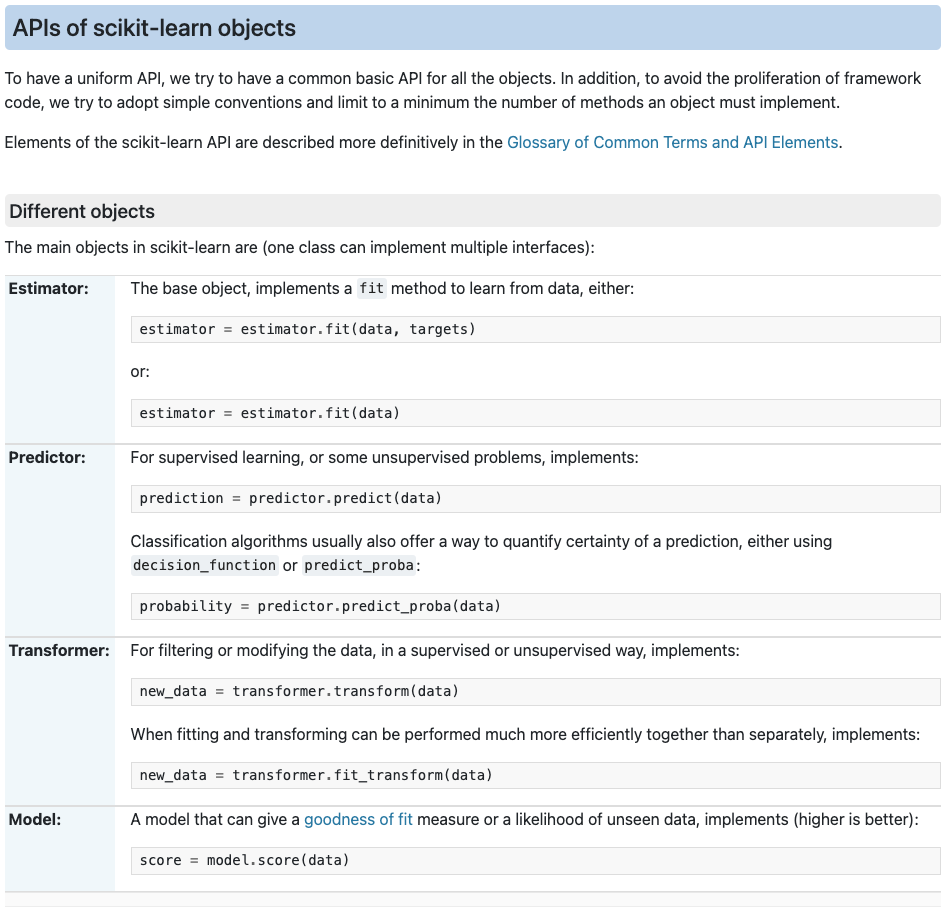
\includegraphics[width=6cm]{data/sklearn_api.png}
            };
        \end{tikzpicture}
        \vfill
    \end{frame}

    \begin{frame}[fragile]{Python: scikit-learn} % Linear regression
        \begin{tikzpicture}
            \node[
                minimum width=\codewidth,
                text width=\codewidth,
                align=left,
                inner sep=0pt,
                anchor=north,
                label={[blue,
                        anchor=north east,
                        font=\ttfamily\fontsize{5}{6}\selectfont,
                        inner sep=0pt,
                        outer sep=0pt,
                        xshift=-3pt,
                        yshift=-3.5pt,
                        text depth=0
                        ]north west:In{[}1{]}:}
            ] (code) at (0, 0) {
                \begin{lstlisting}[style=PythonStyle]
from sklearn.linear_model import LinearRegression

path = '/Users/esten/Downloads/Auto.csv'
df = pd.read_csv(path)

predictors = ['cylinders', 'displacement', 'horsepower',
              'weight', 'acceleration', 'year']
target = 'mpg'

model = LinearRegression()
model.fit(df[predictors], df[target])

# Print model coefficients
print(f'Intercept: {model.intercept_}')
print(f'Coefficients: {model.coef_}')

# Print model residuals
predictions = model.predict(df[predictors])
residuals = df[target] - predictions
print(f'Residuals: {residuals.values[:5]}...')
                \end{lstlisting}
            };

            \node[
                minimum width=\codewidth,
                text width=\codewidth,
                align=left,
                inner sep=0pt,
                anchor=north,
                label={[red,
                        anchor=north east,
                        font=\ttfamily\fontsize{5}{6}\selectfont,
                        inner sep=0pt,
                        outer sep=0pt,
                        xshift=-3pt,
                        yshift=-3.5pt,
                        text depth=0
                        ]north west:Out{[}1{]}:}
            ] (output) at ($ (code.south) - (0, 0.2) $) {
                \begin{lstlisting}[style=PythonOutput]
Intercept: -14.53525048050604
Coefficients: [-3.29859089e-01  7.67843024e-03 -3.91355574e-04 -6.79461791e-03
    8.52732469e-02  7.53367180e-01]
Residuals: [2.91708096 0.92742531 2.46368456 0.46552549 1.71359255]...
                \end{lstlisting}
            };
            \node[] at (4.4, -6.8) {};
            \node[] at (-5.4, -0.1) {};
        \end{tikzpicture}
    \end{frame}

    \begin{frame}[fragile]{Python: scikit-learn} % Support vector regression
        \begin{tikzpicture}
            \node[
                minimum width=\codewidth,
                text width=\codewidth,
                align=left,
                inner sep=0pt,
                anchor=north,
                label={[blue,
                        anchor=north east,
                        font=\ttfamily\fontsize{5}{6}\selectfont,
                        inner sep=0pt,
                        outer sep=0pt,
                        xshift=-3pt,
                        yshift=-3.5pt,
                        text depth=0
                        ]north west:In{[}1{]}:}
            ] (code) at (0, 0) {
                \begin{lstlisting}[style=PythonStyle]
from sklearn.svm import SVR

path = '/Users/esten/Downloads/Auto.csv'
df = pd.read_csv(path)

predictors = ['cylinders', 'displacement', 'horsepower',
              'weight', 'acceleration', 'year']
target = 'mpg'

model = SVR(kernel='linear')
model.fit(df[predictors], df[target])

# Print model coefficients
print(f'Intercept: {model.intercept_}')
print(f'Coefficients: {model.coef_}')

# Print model residuals
predictions = model.predict(df[predictors])
residuals = df[target] - predictions
print(f'Residuals: {residuals.values[:5]}...')
                \end{lstlisting}
            };

            \node[
                minimum width=\codewidth,
                text width=\codewidth,
                align=left,
                inner sep=0pt,
                anchor=north,
                label={[red,
                        anchor=north east,
                        font=\ttfamily\fontsize{5}{6}\selectfont,
                        inner sep=0pt,
                        outer sep=0pt,
                        xshift=-3pt,
                        yshift=-3.5pt,
                        text depth=0
                        ]north west:Out{[}1{]}:}
            ] (output) at ($ (code.south) - (0, 0.2) $) {
                \begin{lstlisting}[style=PythonOutput]
Intercept: [-35.38646279]
Coefficients: [[-1.0526357   0.05910105 -0.03667206 -0.00831565  0.56218046  0.96851648]]
Residuals: [3.0266171  0.62154228 3.10666275 1.34695011 3.07475274]...
                \end{lstlisting}
            };
            \node[] at (4.4, -6.8) {};
            \node[] at (-5.4, -0.1) {};
        \end{tikzpicture}
    \end{frame}

    \def\codewidth{10cm}

    \begin{frame}[fragile]{Coding tips: Separation of concerns} % Spaghetti
        \centering
        \begin{tikzpicture}
            \node[
                minimum width=\codewidth,
                text width=\codewidth,
                align=left,
                inner sep=0pt,
                anchor=north,
                label={[blue,
                        anchor=north east,
                        font=\ttfamily\fontsize{4}{4}\selectfont,
                        inner sep=0pt,
                        outer sep=0pt,
                        xshift=-3pt,
                        yshift=-3.5pt,
                        text depth=0
                        ]north west:In{[}1{]}:}
            ] (code) at (0, 0) {
                \begin{lstlisting}[style=PythonStyle, basicstyle=\ttfamily\fontsize{4}{4}\selectfont]
# Read and clean data
path = '/Users/esten/Downloads/Auto.csv'
df = pd.read_csv(path)

# Split data
train = df.iloc[:int(len(df) * 0.8)]
validation = df.iloc[int(len(df) * 0.8):]

# Define input and output variables
predictors = ['cylinders', 'displacement', 'horsepower',
                'weight', 'acceleration', 'year']
target = 'mpg'

# Define necessary data structures for state
chosen_predictors = []
mses = []

while len(predictors) > 0:
    best_predictor = {'mse': float('inf'), 'predictor': None}

    for predictor in set(predictors) - set(chosen_predictors):
        potential_predictors = chosen_predictors + [predictor]

        # Fit and evaluate model
        model = LinearRegression()
        model.fit(train[potential_predictors], train[target])
        predictions = model.predict(validation[potential_predictors])
        test_mse = np.mean((validation[target] - predictions) ** 2)

        # Compare model with previous best
        if test_mse < best_predictor['mse']:
            best_predictor = {'mse': test_mse, 'predictor': predictor}

    # Update state
    chosen_predictors.append(best_predictor['predictor'])
    mses.append(best_predictor['mse'])
    predictors = [p for p in predictors if p != best_predictor['predictor']]
                \end{lstlisting}
            };
            \node[] at (0, -7.55) {};
        \end{tikzpicture}
    \end{frame}

    \begin{frame}[fragile]{Coding tips: Separation of concerns} % Chunks
        \centering
        \begin{tikzpicture}
            \node[
                minimum width=\codewidth,
                text width=\codewidth,
                align=left,
                inner sep=0pt,
                anchor=north,
                label={[blue,
                        anchor=north east,
                        font=\ttfamily\fontsize{4}{4}\selectfont,
                        inner sep=0pt,
                        outer sep=0pt,
                        xshift=-3pt,
                        yshift=-3.5pt,
                        text depth=0
                        ]north west:In{[}1{]}:}
            ] (code) at (0, 0) {
                \begin{lstlisting}[style=PythonStyle, basicstyle=\ttfamily\fontsize{4}{4}\selectfont]
# Read and clean data
path = '/Users/esten/Downloads/Auto.csv'
df = pd.read_csv(path)

# Split data
train = df.iloc[:int(len(df) * 0.8)]
validation = df.iloc[int(len(df) * 0.8):]

# Define input and output variables
predictors = ['cylinders', 'displacement', 'horsepower',
                'weight', 'acceleration', 'year']
target = 'mpg'

# Define necessary data structures for state
chosen_predictors = []
mses = []

while len(predictors) > 0:
    best_predictor = {'mse': float('inf'), 'predictor': None}

    for predictor in set(predictors) - set(chosen_predictors):
        potential_predictors = chosen_predictors + [predictor]

        # Fit and evaluate model
        model = LinearRegression()
        model.fit(train[potential_predictors], train[target])
        predictions = model.predict(validation[potential_predictors])
        test_mse = np.mean((validation[target] - predictions) ** 2)

        # Compare model with previous best
        if test_mse < best_predictor['mse']:
            best_predictor = {'mse': test_mse, 'predictor': predictor}

    # Update state
    chosen_predictors.append(best_predictor['predictor'])
    mses.append(best_predictor['mse'])
    predictors = [p for p in predictors if p != best_predictor['predictor']]
                \end{lstlisting}
            };
            \node[
                anchor=north west,
                fill=purple,
                inner sep=0pt,
                outer sep=0pt,
                minimum width=\codewidth,
                minimum height=2.78cm,
                opacity=0.2,
                align=right,
            ] (setup) at ($ (code.north west) + (0.01, -0.01) $) {};
            \node[anchor=north east, inner sep=2pt] at (setup.north east) {\textcolor{red}{\tiny{Setup}}};

            \node[
                anchor=north west,
                fill=green,
                inner sep=0pt,
                outer sep=0pt,
                minimum width=\codewidth,
                minimum height=3.478cm,
                opacity=0.2
            ] (selection) at (setup.south west) {};
            \node[anchor=north east, inner sep=2pt] at (selection.north east) {\textcolor{green}{\tiny{Selection}}};

            \node[
                anchor=north west,
                fill=blue,
                inner sep=0pt,
                outer sep=0pt,
                minimum width=\codewidth - 0.8cm,
                minimum height=1cm,
                opacity=0.2
            ] (training) at ($ (selection.north west) + (0.66, -0.98) $) {};
            \node[anchor=north east, inner sep=2pt] at (training.north east) {\textcolor{blue}{\tiny{Modelling}}};

            \node[
                anchor=north west,
                fill=orange,
                inner sep=0pt,
                outer sep=0pt,
                minimum width=\codewidth - 0.48cm,
                minimum height=0.83cm,
                opacity=0.2
            ] (state) at ($ (selection.north west) + (0.34, -2.6) $) {};
            \node[anchor=north east, inner sep=2pt] at (state.north east) {\textcolor{orange}{\tiny{Housekeeping}}};
            \node[] at (0, -7.55) {};
        \end{tikzpicture}
    \end{frame}

    \begin{frame}[fragile]{Coding tips: Separation of concerns} % Proper
        \begin{tikzpicture}
            \node[
                minimum width=\codewidth,
                text width=\codewidth,
                align=left,
                inner sep=0pt,
                anchor=north,
                label={[blue,
                        anchor=north east,
                        font=\ttfamily\fontsize{4}{4}\selectfont,
                        inner sep=0pt,
                        outer sep=0pt,
                        xshift=-3pt,
                        yshift=-3.5pt,
                        text depth=0
                        ]north west:In{[}1{]}:}
            ] (code) at (0, 0) {
                \begin{lstlisting}[style=PythonStyle, basicstyle=\ttfamily\fontsize{4}{4}\selectfont]
# Read and clean data
path = '/Users/esten/Downloads/Auto.csv'
df = pd.read_csv(path)

# Split data
train = df.iloc[:int(len(df) * 0.8)]
validation = df.iloc[int(len(df) * 0.8):]

# Define input and output variables
predictors = ['cylinders', 'displacement', 'horsepower',
                'weight', 'acceleration', 'year']
target = 'mpg'

# Define necessary data structures for state
chosen_predictors = []
mses = []

def fit_and_evaluate_model(model: LinearRegression, train: pd.DataFrame,
                           validation: pd.DataFrame, variables: List[str],
                           target: str):
    """ Fit a given model on a training dataset using a given set of variables
    and return MSE from a validation dataset. """
    model = LinearRegression()
    model.fit(train[potential_predictors], train[target])
    predictions = model.predict(validation[potential_predictors])

    return np.mean((validation[target] - predictions) ** 2)

while len(predictors) > 0:
    best_predictor = {'mse': float('inf'), 'predictor': None}

    for predictor in set(predictors) - set(chosen_predictors):
        potential_predictors = chosen_predictors + [predictor]
        test_mse = fit_and_evaluate_model(LinearRegression(), train, validation,
                                            variables=potential_predictors,
                                            target=target)

        # Compare model with previous best
        if test_mse < best_predictor['mse']:
            best_predictor = {'mse': test_mse, 'predictor': predictor}

    # Update state
    chosen_predictors.append(best_predictor['predictor'])
    mses.append(best_predictor['mse'])
    predictors = [p for p in predictors if p != best_predictor['predictor']]
                \end{lstlisting}
            };
            \node[
                anchor=north west,
                fill=blue,
                inner sep=0pt,
                outer sep=0pt,
                minimum width=\codewidth - 0.14cm,
                minimum height=1.8cm,
                opacity=0.2
            ] (training) at ($ (code.north west) + (0.07, -2.8) $) {};
            \node[anchor=north east, inner sep=2pt] at (training.north east) {\textcolor{blue}{\tiny{Modelling}}};

            \node[
                anchor=north west,
                draw=blue,
                line width=0.5pt,
                inner sep=0pt,
                outer sep=0pt,
                minimum width=\codewidth - 1.37cm,
                minimum height=0.52cm
            ] (training) at ($ (code.north west) + (0.74, -5.49) $) {};

            \node[] at (0, -7.55) {};
        \end{tikzpicture}
    \end{frame}

    \begin{frame}{Regularization: Motivation}
        \centering
        \vfill
        \begin{tikzpicture}
            \node[draw=black, fill=white] {
                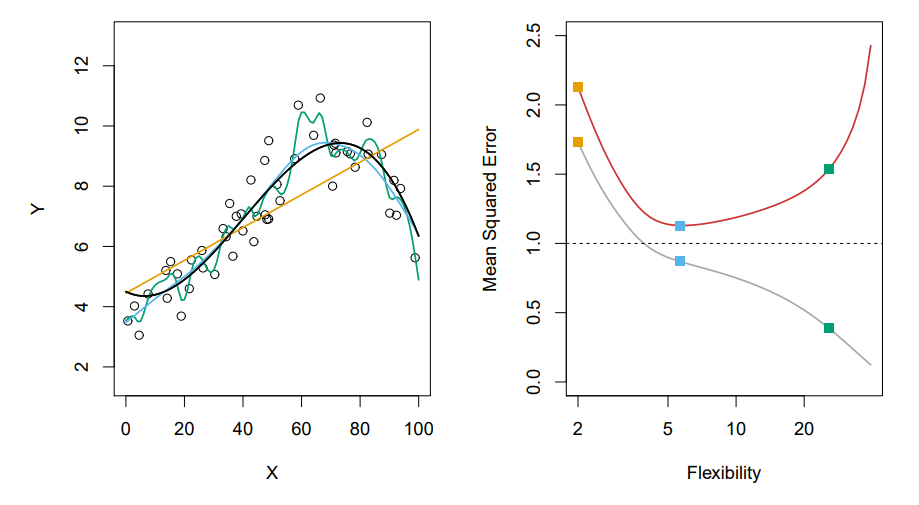
\includegraphics[width=8cm]{data/overfitting.png}
            };
        \end{tikzpicture}
        \vfill
    \end{frame}

    \begin{frame}{Regularization: Out-of-sample testing}
    \end{frame}

    \begin{frame}{Regularization: Methods}
        \begin{enumerate}
            \item Variable selection
            \begin{enumerate}
                \item[a.] Best subset selection
                \item[b.] Forward stepwise selection
                \item[c.] Backward stepwise selection
            \end{enumerate}
            \item Shrinkage
            \begin{enumerate}
                \item[a.] LASSO
                \item[b.] Ridge Regression
                \item[c.] Elastic net
            \end{enumerate}
            \item Dimensionality reduction
            \begin{enumerate}
                \item[a.] Principal Component Regression
                \item[b.] Partial Least Squares
            \end{enumerate}
        \end{enumerate}
    \end{frame}

    \begin{frame}[t]{Variable selection: Outline}
        \underline{Problem}\\
        We have a set of predictors $P=\{x_0, x_1, ...\}$ and a target variable $y$, and we want to find the subset $p \subseteq P$ that yields the best (linear) model for predicting $y$.\\
    \end{frame}

    \begin{frame}[t]{Variable selection: Outline}
        \underline{Problem}\\
        We have a set of predictors $P=\{x_0, x_1, ...\}$ and a target variable $y$, and we want to find the subset $p \subseteq P$ that yields the best (linear) model for predicting $y$.\\
        \vspace{1cm}
        \underline{Motivation}\\
        \begin{enumerate}
            \item Simplify interpretation
            \item Reduce model complexity (overfitting)
        \end{enumerate}
    \end{frame}

    \begin{frame}[t]{Variable selection: Outline}
        \underline{Problem}\\
        We have a set of predictors $P=\{x_0, x_1, ...\}$ and a target variable $y$, and we want to find the subset $p \subseteq P$ that yields the best (linear) model for predicting $y$.\\
        \vspace{1cm}

        \begin{tikzpicture}

        \end{tikzpicture}
    \end{frame}

    \begin{frame}[t]{Variable selection: Best subset selection}
        \underline{Problem}\\
        We have a set of predictors $P=\{x_0, x_1, ...\}$ and a target variable $y$, and we want to find the subset $p \subseteq P$ that yields the best (linear) model for predicting $y$.\\
        \vspace{1cm}
        \underline{Solution (best subset selection)}\\
        Train models on all subsets $p$ and select the best one.
    \end{frame}

    \begin{frame}[t]{Variable selection: Best subset selection}
        \underline{Problem}\\
        We have a set of predictors $P=\{x_0, x_1, ...\}$ and a target variable $y$, and we want to find the subset $p \subseteq P$ that yields the best (linear) model for predicting $y$.\\
        \vspace{1cm}
        \underline{Solution (best subset selection)}\\
        Train models on all subsets $p$ and select the best one.
    \end{frame}

     \begin{frame}{Variable selection: Best subset selection}
     \end{frame}

%     \begin{frame}{Variable selection: Forward stepwise selection}
%     \end{frame}

%     \begin{frame}{Variable selection: Backward stepwise selection}
%     \end{frame}

%     \begin{frame}{Regularization: Outline}
%     \end{frame}

%     \begin{frame}{Regularization: Feature standardization}
%     \end{frame}

%     \begin{frame}{Regularization: Ridge regression}
%     \end{frame}

%     \begin{frame}{Regularization: Lasso}
%     \end{frame}

%     \begin{frame}{Regularization: Elastic net}
%     \end{frame}

%     \begin{frame}{Dimensionality reduction: Outline}
%     \end{frame}

%     \begin{frame}{Dimensionality reduction: Principal component analysis}
%     \end{frame}

%     \begin{frame}{Dimensionality reduction: Principal component regression}
%     \end{frame}

%     \begin{frame}{Dimensionality reduction: Partial least squares}
%     \end{frame}
\end{document}
